% !TEX root = twibop2.tex

\chapter{Control and Self-control}
\epigraph{Cybernetics penetrated and continues to penetrate every area of man's work and daily life. This is the science of the optimal control over complex processes and systems.}  {A.I. Berg}

\section{The Problem of Control}

\txthead{Control against disorganization.} Although the world around us is full of
chance, it nonetheless proves to be organized and ordered in many
ways. \redem{The disorganizing effect of chance is countered by the organizing
influence of control and self-control.}

Suppose an airplane flies from Moscow to Leningrad. Various
random factors affect it during the flight. Therefore, all three space
coordinates of the airplane are random functions of time. The flight
trajectory is a realization of these random functions. However, these
``subtleties'' do not bother the passengers; they fasten their belts before
takeoff confident that whatever thunderstorms might occur on the way
and whichever winds affect the airplane, it will arrive at Leningrad
airport. The basis for this confidence lies in the aircraft's control system
and the actions of the pilot. We met queueing systems above, and although
there is a great deal of chance, they comply with their objectives.
This is because the organization of the system and the control of
its operation is well-designed.

\redem{Controls} take on a variety of guises. Suppose we want a set of books
to serve public for a long time. This is impeded by chances both purely
physical in nature and those related to the attitudes of some readers. So
we control matters: we take care of the binding, regulate the
temperature, humidity, and illuminance in the rooms where the books
are stored, give the book a library card, and set up the rules governing
the use of the books.

No one is safe from disease, and although each disease has a definite
cause, the prevalence and lethality of a disease on the scale, say, of
a town is governed by chance. When fighting it, we must control matters
by improving working and living conditions, taking preventive medical
measures, constructing stadiums, swimming pools, sport complexes,
ordering pharmacies to supply the necessary drugs, etc.

Thus, there is a \redem{confrontation} of two powerful factors in the world,
two basic trends. On the one hand, there is \redem{randomness}, a tendency to
disorganization, disorder, and destruction in the long run. On the other
hand, there is \redem{control} and self-control, a tendency to organization, order, development, and progress.

\txthead{Choice as a prerequisite of control.} If all the processes and
phenomena in the world were strictly predetermined, it would be
meaningless even to speak of the possibility of control. \redem{In order to
control something, there must be some choice.} How may we make
a decision if everything is predetermined in advance? Every
phenomenon must have several probable lines of development. One may
say that a world built on probability is the only world in which control
is possible.

Control acts against chance, even though the possibility of control is
brought about by the existence of chance. It is random occurrences that
help us avoid predetermination. We can say that randomness ``brings to
life'' its own ``grave-digger'', i. e. control. This is a manifestation of the
dialectic unity of the necessary and the random in the real world.

\txthead{Control and feedback.} Two different control schemes are shown in
\figr{control-scheme-1} , where $S$ is the controlled system, $CU$ is the control unit, $V$ is the input to the controlled system (the control signal), $P$ are random perturbations affecting the controlled system, and $w$ is the final output
from the system. Scheme $(b)$ differs from scheme $(a)$ in having a feedback
loop, that is the control unit receives information about the results of
control.
\begin{figure}[!ht]
 \centering
 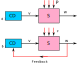
\includegraphics[width=0.75\tfwidth]{figures/control-scheme-1.pdf}
\caption{Two different control schemes.\label{control-scheme-1}}
%fig 3.1
 \end{figure}

What is feedback for? In answering this question, let me remark that
the ``relationship'' between randomness and control is one of active
confrontation. Control acts against chance, and chance acts against
control. The latter fact requires flexible control, the possibility for
adjustment. The control unit must be able continuously to receive data
about the results of the control and correct its signals to the system
appropriately.

In point of fact, any real control system supposes the presence of
a feedback loop. \redem{Control without feedback is not only ineffective, it is
actually unviable.}

Take for example someone driving a motor-car. Imagine for a minute
that the feedback suddenly disappeared, that is, the driver stopped
attending to the motion of the car. The car would continue to be
controlled, but without any feedback. The car is immediately affected by
a variety of random events. A small bump or bend in the road, a car
moving in the opposite direction all are random and could lead to an
accident in only a few seconds.

\txthead{The control algorithm.} Now what should be done and how should the system be controlled? It depends on the situation and the goal being
pursued. In fact the answer lies in the algorithm of control. 
\begin{mybox}{}
A control algorithm is a sequence of actions that must be carried out to reach a set of goals.
\end{mybox}

In the example with the car and a driver, the control algorithm
contains rules on how to start the engine, how to brake, how to turn,
how to shift gears, and so on. The algorithm also contains the traffic
regulations and good driving practice.

In some cases the control algorithm is simple. For instance, in order
to use a coffee machine, only the following two actions need be carried
out: put a coin in the slot, and press the appropriate buttons. This is the
complete control algorithm for this machine. In other cases, the control
algorithm is much more complicated. For instance, it is more difficult to
drive a car, while flying a jet is even more complicated. In very
complicated cases, the control algorithm cannot even be defined in full.
For instance, complete control algorithms for managing a large
enterprise or industry simply do not exist.

\section{From the ``Black Box'' to Cybernetics}

Despite the diversity of algorithms, the processes of control can be
investigated from general positions, irrespective of the details of the
considered system. A typical example is the simulation of a system using
the ``black box'' model.


\txthead{What is a ``black box''?} Suppose we consider a controlled system,
where $V_{1}, V_{2}, \ldots , V_{m}$ are its inputs (control signals), $P$ is a random perturbation, and $W_{1}, W_{2}, \ldots , W_{n}$ are its outputs (Figure \ref{black-box-1}). Now let us suppose that we do not know or do not care what is inside the system. We only need investigate the relationships between the inputs ( $V_{1}, V_{2}, \ldots , V_{m}$) and the outputs ($W_{1}, W_{2}, \ldots , W_{n}$). It is said in this case that the given system is a ``black box''.

\begin{figure}[!ht]
 \centering
 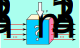
\includegraphics[width=0.8\tfwidth]{figures/black-box-1.pdf}
\caption{A black box is a system whose inputs and outputs are known, but internal structure is not.\label{black-box-1}}
% fig 3.2
 \end{figure}
 
Any controlled system is a ``black box'' if its internal structure is not
considered, and only the responses of the outputs to the inputs are
investigated.



\txthead{Man surrounded by black boxes.} The advance of science and
technology has surrounded mankind by a vast number of controlled
systems. As a rule, we are not a bit bothered by this because we quickly
get accustomed (sometimes unconsciously) to considering these systems
as black boxes. We find out how, what, and where to turn, press, or
switch the buttons to obtain the desired effect. If you want to watch
a TV show, there is no need to know the structure or workings of
a television. We need only press the proper button and select the
channel. To make a telephone call, we do not have to be telephone
engineers; we just pick up the receiver, wait for the call signal, and dial
the telephone number. We use television, telephone, and many other
systems and consider them to be black boxes. Naturally, we could learn
what is inside the system and how it works if we want to, but in our
modern world we often think it's a waste of time to study what we can
quite do without in practice. More and more often we prefer to use
black boxes and when they fail we call in a professional technician.

We should recognize the validity of the complaints that as modern
people we have become less curious, that we do not want to see things
in depth because there are too many things to see, and it is not difficult
to use them. However, I should not make things appear to be worse
than they are. Firstly, there is a system of universal secondary education
at least in the developed countries, which ensures each person has
a basic minimum knowledge. Secondly, from the viewpoint of the
development of society, the knowledge available to the society
as a whole is more important than what a single person may
know.

\txthead{Complex systems as black boxes.} Modern systems are becoming more
and more sophisticated as their functional capacities become more and
more diverse. Naturally, the more we need to know about the functions
of a system, the further we push our investigation of its inner structure
into the background, and in many cases such a total investigation would
prove infeasible because of the complexity of the system.

This shift of emphasis leads us to a qualitatively new viewpoint, in
which the main aim is to investigate control and self-control as general
processes irrespective of the concrete devices comprising the systems.
This point of view brings about \redem{cybernetics} as the science of control
(self-control) in complex systems.

Curiously this point of view reveals an interesting fact and makes us
look at the black-box model in another way. It turns out that we do not
need understand every structural subtlety of a complex system, indeed
its separation into component parts can obscure essential information.
The black-box model becomes \redem{fundamental} as the only acceptable way
of analyzing a complex system.

\txthead{What is cybernetics?} The science of cybernetics was founded by the American scientist Norbert Wiener (1894-1964) and dates from 1948
when he published his famous book \redem{Cybernetics, or Control and
Communication in the Animal and the Machine}. Wiener wrote:
\begin{quote}
``We have decided to call the entire field of control and
communication theory, whether in the machine or in the animal, by the
name cybernetics, which we form from the Greek $\varkappa \upsilon \beta \epsilon \rho \nu  \eta \tau \eta \zeta$, or steersman.''\\[-10pt]
\end{quote}
It should be noted that the term ``cybernetics'' was not new. Plato
used it meaning the art of controlling ships. The French physicist
Amp\'ere classified sciences in the first half of the $19^{\text{th}}$ century and placed a science, which was the study of the methods of government, in section
83. Amp\'ere called this science cybernetics. Today we only use the term
``cybernetics'' in the sense given to it by Wiener. 
\begin{mybox}{}
Cybernetics is the science of the control and communication in complex systems, be they machines or living organisms.
\end{mybox}

The Soviet scientist L.A. Rastrigin wrote a book called \redem{This Chancy,
Chancy, Chancy World} (Mir Publishers, Moscow, 1984), in which he
remarked:
\begin{quote}
``Until cybernetics made its appearance, control processes in an
electric generator were investigated by electrical engineering, control of
the motion of a clock pendulum (in effect a swing) was dealt with in
mechanics, and control of population dynamics in biology. Norbert
Wiener was the first to point to the universal nature of control and to
show that the organizing of an object (the lowering of its entropy) could
be achieved by means of standard procedures, that is, by applying the
methods of cybernetics independently of the physical characteristics of
the object."
\end{quote}
L.A. Rastrigin imaginatively calls cybernetics a science which fights
randomness, thus emphasizing the idea of control counteracting
disorganization and destruction caused by diverse random factors.

\txthead{Cybernetics and robots.} One of the central topics of cybernetics
concerns \redem{process automation}, in particular, \redem{self-control in complex systems}. Investigations into this area resulted in the appearance of a discipline called ``robotics''. Modern cybernetics literature discusses the possibility of designing automata that can reproduce and teach themselves.
Artificial intelligence is also a topic being investigated. The following
questions are being studied: Is the machine capable of creativity? Could
a machine become cleverer than its designer? Could the machine think?

The more sophisticated types of robots are still in the realms of
science fiction, although we often hear discussions about the possibilities
of robotics, or rather whether artificial ``men'' might be possible. The
layman now seems to believe that cybernetics is indeed simply the
science of robots, automata, or thinking machines. The true purpose of
cybernetics as the science of control is now masked by the fantastic
technological promise.

True, cybernetics does include the problems of automation, and thus
contributes to scientific and technological progress. The automation of
various processes, the design of automatic Lunar explorers, automatic
space docking are all achievements of cybernetics. Cybernetics also
investigates computer creativity and artificial intelligence. However, this
is not so as to evolve an artificial person. When we programme
computers to ``compose'' music or ``write'' a poem or play chess or give
a ``talk'', we are attempting to simulate creativity and so find out more
about these processes. It could be said that we are investigating the limit
of computer abilities, but not that we want to substitute them for
human beings in the future: we just want to understand several
important topics thus making it possible to go deeper into the control
processes occurring in human beings. The reader should remember this
and not consider cybernetics to be just the ``science of robots''.

We may now start discussing the central notion of cybernetics, i. e.
\redem{information}. Let me say right away that cybernetics investigates control
and self-control primarily from the viewpoint of information. It
investigates the collection, conversion, transmission, storage, and
retrieval of information. In a certain sense of the word, cybernetics can
be regarded as the ``science of information''.

\section{Information }

Let me begin with an excerpt from the immortal poem \redem{De Rerum
Natura} (On the Nature of Things) by Carus Lucretius (ca. 99-55 B.C.):
\begin{quote}
`` \ldots if things came to being from nothing,\\
Every kind might be born from all things,\\
Nought would need a seed.\\
First men might arise from the sea, and from the land,\\
The race of scale creatures, and birds burst forth \\
The sky. Cattle and other herds, and all the tribe\\
Of wild beasts with no law of birth,\\
Would haunt tilth and desert \ldots ''
\end{quote}
It is interesting that there is here a hint of the conservation of not
only matter and energy, but also of something else, which is neither
matter nor energy. There is no shortage of energy and matter in the sea,
but people do not appear in the sea. Nor too does the dry land produce
fish. Truly, ``if things came to being from nothing, \ldots{} nought would need
a seed''. In the modern terminology of science, we might say that this is
a hint of the \redem{conservation of information}. The information needed by
plants and animals to live and reproduce cannot appear ``from nothing''.
It is stored in ``seeds'' and thus handed down from generation to
generation.

The term ``information'' is now encountered everywhere in science and
everyday life. In fact, every activity is related to the \redem{collection,
conversion, transmission, storage, and retrieval of information}. We live in
a world filled with information, and our very existence is impossible
without it. Academician A.I. Berg once said: ``Information penetrates
every pore of the life of human beings and their societies \ldots{} Life is
impossible in a vacuum of either mass-energy or information.''


\txthead{The bit, the unit of information.} What is information? What units is it
measured in? Let us start with a simple example. A train approaches
a station. By remote control, a signalman can switch a train from one
track $(A)$ to another $(B)$. If the switch is up, the train goes along track $A$, and if it is down, the train goes along track $B$. Thus, the signalman, by
moving the switch up or down, is sending a control signal containing
1 bit of information. The word ``bit'' is an abbreviation of ``binary digit''.

To see what we mean by ``binary digit'', recall how digits are used to
write numbers. We commonly use the decimal number system, i.e.
a system with ten digits (0, 1, 2, \ldots , 9). Take a number written in the
\redem{decimal} system, say 235. We say ``two hundred and thirty five'' and, as
a rule, do not pause to think that this means the sum of two hundreds,
three tens, and five units, i. e. $2 \times 10^{2} + 3 \times 10 + 5 \times 10^{0}$. The same number (235) can also be in the \redem{binary} system, which only has two digits, 0 and 1, as 11101011, which means $1 \times 2^{7} + 1 \times 2^{6} + 1 \times 2^{5} + 0 times 2^{4} + 1 \times 2^{3} + 0 \times 2^{2} + 1 \times 2^{1} + 1 times 2^{0}$. Since $2^{7} = 128, \, 2^{6} = 64, \, 2^{5} = 32, \, 2^{3} = 8, 2^{1} = 2, \,\, \text{and} \,\, 2^{0} = 1$, we have our number $128 + 64 + 32 + 8 + 2 + 1 = 235$. Any number can be written in either the
decimal or the binary system. If you don't follow this explanation try
looking at \figr{binary-conversion}.

\begin{figure}[!ht]
 \centering
 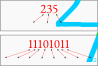
\includegraphics[width=0.75\tfwidth]{figures/binary-conversion.pdf}
\caption{Representing the number 235 in decimal and binary systems.
\label{binary-conversion}}
% fig 3.3
 \end{figure}

Let us return to the railway example. Remember we have two choices:
the switch is either up (track $A$) or down (track $B$). We could write the
digit 0 for switch up and digit 1 for switch down. It can be said that the
control signal can thus be coded by one of the two binary digits, zero or
unity. The signal thus contains one binary digit, or 1 bit of information.

Consider a more interesting example. The railway lines near a station
are shown in \figr{railway-switches}. 

\begin{figure}[!ht]
 \centering
 \includegraphics[width=0.8\tfwidth]{figures/railway-switches.pdf}
\caption{Controlling railway lines by using switches.\label{railway-switches}}
% fig 3.4
 \end{figure}

The railway switches are labelled by the letters $a, \,
b, \, c, \, d, \, e, \, f$, and $g$. If a switch receives a control signal of 0, it opens the left-hand track, and if it receives a signal of 1, it opens the right-hand
track. The signalman has three control switches: the first one sends
a signal (0 or 1) to railway switch $a$, the second one sends a signal
simultaneously to switches $b$ and $c$, and the third one simultaneously to
switches $d, \, e, \, f,$ and $g$. The station has eight tracks: $A, B, C, D, E, F, G,$ and $H$. To send a train along track $A$, all three control switches must be turned to the 0 position, i.e. send the three-digit signal 000. To direct
a train to track $B$, it is necessary to send the three-digit signal 001. Each
track thus has its own three-digit signal, i.e.
\begin{center}
\setlength\arrayrulewidth{0.75pt}\arrayrulecolor{Tomato}
\begin{tabular}{cccccccc}
\toprule
A & B & C & D & E & F & G & H\\
\midrule
000 & 001 & 010 & 011 & 100 & 101 & 110 & 111 \\
\bottomrule
\end{tabular}
\end{center}

We see that to select one of the eight outcomes requires a set of
elementary signals, each of which carries 1 bit of information. Therefore,
to choose a track in this example requires three bits of information.

Thus, in order to select one option out of two, 1 bit of information is
required; in order to select one option out of eight, 3 bits of information
are required. In order to select one of $N$ options, $I$ bits of information
are required, where
\begin{equation}%
I = \log_{2} N.
\label{eq-3.1}
\end{equation}
This is the \redem{Hartley formula}. It was suggested in engineer Ralph Hartley, who was interested information.

\txthead{The Bar Kohba game.} A rebellion against Romans broke in 135 A. D.
in the ancient Judea led by one Bar Kohba. As the legend has it, Bar
Kohba sent a spy into the camp of Romans, and the spy discovered
a great deal before being caught. He was tortured and his tongue was
cut out. However, the spy managed to escape, but without his tongue he
could not report what he had found out in the enemy's camp. Bar
Kohba resolved the problem by asking the spy questions that only
required a ``yes'' or `no'' answer (it was only necessary to nod or shake
the head). Bar Kohba was able to obtain all the information he wanted
from his spy, even though the spy had no tongue.

A similar situation is described in \redem{Le comte de Monte Christo} by
Alexandre Dumas p\'ere. An old man in the novel had been paralyzed
and could neither speak nor move his hands. Nonetheless, his relatives
were able to communicate with him asking him questions which
required only a ``yes'' or a ``no''. If ``yes'', the old man would close his
eyes; if he blinked several times, it was ``no''.


It turns out that any information can be transmitted in the form of
``yes'' and ``no'' answers if the questions are constructed \redem{properly}. This idea underlies the \redem{Bar Kohba game}, which first appeared at the turn of the century in Hungary and then spread to other countries. A player
thinks of something. He may, for instance, make a wish or even think
up a sentence. The other player must guess the wish or sentence by
asking questions, which must be honestly answered. However, the
questions may only require a ``yes'' or ``no'' answer. The quantity of
information needed for a correct guess can be measured by the number
of questions, given that the most rational method of interrogation is
used. Each answer can be enciphered by a binary digit, for instance, we
could use a one for a ``yes'' and a zero for a ``no''. Then the information
needed for a correct guess would be a combination of zeroes and unities.

Let us play a Bar Kohba game with the railway signalman at the
station whose tracks are given in \figr{railway-switches}. The signalman thinks of a track along which a train should travel to the station. We want to
guess the track. The game would go as follows.
\begin{dialogue}
\ques Should switch $a$ open the track on the right?
\ans No. (let us cipher this answer by digit 0).
\ques Should switch $b$ open the track on the right?
\ans Yes (we cipher: 1). 
\ques Should switch $e$ open the track on the right? 
\ans Yes (we cipher: 1).
\end{dialogue}
Having asked these three questions, we see that the signalman decided
on track $D$. The information needed to answer was the chain of answers
``no-yes-yes'' or, in other words, by the set of binary digits 011. We
know that the information capacity of the signalman's ``riddle'' was three
bits long. Each of the signalman's three answers contained one bit of
information.

Let me cite one more example of the Bar Kohba game. There are 32
pupils in a class. The teacher decides on one of them. How can we find
out which one? Let us take the class register, in which the surnames of
all the pupils are listed in alphabetical order and enumerated. Let us
start asking questions.
\begin{dialogue}
\ques Is the pupil among those listed from 17 to 32? 
\ans Yes (we cipher: 1).
\ques Is the child among those listed from 25 to 32?
\ans No (0). 
\ques Is the child among those listed from 21 to 24?
\ans No (0). 
\ques Is the child among those listed either 19 or 20?
\ans Yes (1).
\ques Is it number 20?
\ans No (0).
\end{dialogue}
Consequently, the teacher meant pupil number 19 in the class register.
This information required the chain of answers ``yes-no-no-yes-no'' or, in
other words, the set of binary digits 10010. It is clear from \figr{32-pupils} that the area in which the surname was searched for gradually decreased
with each answer. To solve the problem, it only required to ask five
questions. According to the Hartley formula, the selection of the option
out of 32 requires log, $3^{2} = 5$ bits of information. Therefore, each of the
answers in this game contained 1 bit of information.
\begin{figure}[!ht]
 \centering
 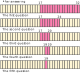
\includegraphics[width=0.85\tfwidth]{figures/32-pupils.pdf}
\caption{Finding out the selected pupil from a group of 32.\label{32-pupils}}
% fig 3.5
 \end{figure}

Perhaps I have created the impression that each answer in the Bar
Kohba game always contains 1 bit of information. It is easy to see that
this is not so. Suppose that we established that a surname was listed
from 17 to 32 and then ask: Is it the surname listed from 9 to 16? It is
dear that the answer to this question must be negative. The fact that the
answer is obvious means that it does not contain any information at all.
Naturally, we might have a situation without ``silly'' questions.
\begin{dialogue}
\ques Is the surname listed from 1 to 8?
\ans No.
\ques Is it listed from 25 to 32?
\ans No.
\ques Is it listed from 9 to 16?
\ans No.
\ques Is it listed from 17 to 24?
\ans Yes.
\ques Is it listed either 23 or 24?
\ans No.
\ques Is it listed either 19 or 20?
\ans Yes.
\ques Is it listed 19?
\ans Yes.
\end{dialogue}
Having chosen this strategy, we extracted the needed information
using eight questions rather than five. The quantity of information in the
final answer equals 5 bits as before. Therefore, each individual answer in
this case contained, on the average, 5/8 bit of information.

Thus, we see that ``yes-no'' answers do not always contain 1 bit of
information. Running ahead of ourselves, we can note that 1 bit is the
\redem{maximum} information that such an answer may contain.

``Just a minute,'' you might say, ``if this is so, does then a binary digit
not always carry one bit of information?''

``Quite true,'' I would answer.

``Then how about the definition of a bit of information given above?
Can we use the Hartley formula?''

All that has been said about a bit of information (and about the
Hartley formula) remains valid, although with a reservation that \redem{every
option should be equally probable}. I did not want to discuss this topic too
early, but now the time has come to do so.

\txthead{Information and probability. The Shannon formula.} I have
emphasized that control is only possible in a world where necessity is
dialectically confronted with chance. In order to control something,
there must be choice. Any situation we want to control carries with it
uncertainty. This uncertainty can be compared with a shortage of
information. While we control an object, we introduce information and
thus decrease the uncertainty.

For instance, a train may arrive along any of the eight tracks in our
example above, so there is uncertainty. By sending a control signal with
three bits of information, the signalman eliminates this uncertainty, and
the train is directed along one particular track. The teacher could have
thought of any of his 32 pupils, so there was uncertainty which surname
had been chosen. Having listened to the answers for a number of
questions with an overall quantity of information of five bits, we can
eliminate this uncertainty and identify the pupil.

Now let us return to the starting point of our reasoning and to the
presence of choice. Until now, we assumed that each option was equally
probable. The signalman could have chosen any of the eight tracks with
equal probability. The teacher could have picked anyone of his 32
pupils. However, we often have to choose between options that are not
equally probable, and then it is necessary to pay due attention to the
\redem{probability associated with each option}. Suppose the answer to a question may be either ``yes'' or ``no'' and both outcomes are equally probable.
The answer then will carry precisely 1 bit of information. However, if
the ``yes'' or ``no'' outcomes have different probabilities, then the answer
will contain less than 1 bit of information. And the greater the difference
between the probabilities of the two outcomes, the smaller the quantity
of information. In the limit of the probability of a ``yes'' (or a ``no'')
being unity, the answer will not contain any information at all.

Now, let us look at what happens when different outcomes (different
options) have different probabilities. I do not want to cram this book
with mathematics, so I shall only discuss the basic results. Suppose $\xi$ is
a random discrete variable that may assume the values $x_{1}, x_{2}, x_{3},\ldots{} , x_{N}$ with probabilities  $p_{1}, p_{2}, p_{3},\ldots{} , p_{N}$, respectively. We have $N$ outcomes ($N$ different values of the random variable) which appear with different probabilities. Given an observation of the variable $\xi$ and its value, how much information does this observation carry?

This problem was investigated by the American scientist Claude
Shannon in the mid-1940s. He came to the conclusion that we obtain
the quantity of information equal (in bits) to
\begin{equation}%
I(\xi) = \sum_{i=1}^{N} p_{i}  \log_{2} \frac{1}{p_{i}}.
\label{eq-3.2}
\end{equation}
This is a fundamental relation in information theory. It is called the
\redem{Shannon formula}.

Suppose that the outcomes are equally probable, and the random
variable may take on the values $x_{i}$ with the same probability $p$. This
probability is clearly $1/N$ and so from \eqref{eq-3.2} we obtain
\begin{equation*}%
I =  \frac{1}{N} \, \sum_{i=1}^{N}   \log_{2} \, N = \frac{1}{N} \, N \,  \log_{2} N =   \log_{2} \, N,
%\label{shannon-formula}
% eq 3.2
\end{equation*}
i.e. the Hartley formula \eqref{eq-3.1}. Consequently, we see that the Hartley formula is a special case of the Shannon formula when all outcomes are
equally probable.

Using the Shannon formula, let us find how much information can be
contained in a ``yes'' or ``no'' answer. Suppose $p$ is the probability of
a ``yes''. Then the probability of a ``no'' answer is $1 - p$. According to
\eqref{eq-3.2}, the information obtained from the answer to a question is
\begin{equation}%
I = p \ \log_{2}  \frac{1}{p} + (1 - p)   \log_{2} \frac{1}{1-p}.
\label{eq-3.3}
% eq 3.3
\end{equation}
The graph of $I$ versus $p$, as defined by \eqref{eq-3.3}, is given in \figr{shannon-distro}.


Maximum information (1 bit) is obtained when $p = 1/2$, i.e. when
a ``yes'' and a ``no'' are equally probable. Now we can refine our notion
of ``1 bit of information''. \redem{This is the information contained in a digit that may take on only two values provided both values are equally probable}.

It follows that the best strategy in the Bar Kohba game is to ask
``yes'' or ``no'' questions, the answers to which are nearly or equally
probable. Recall the question: ``Is the surname listed from 17 to 32?''
Here the answers ``yes'' and ``no'' are equally probable because there are
32 pupils and the numbers from 17 to 32 cover half of the pupils. Therefore,
the answer to this question gives 1 bit of information. But for the
question: ``Is the surname listed from 1 to 8?'' the range of numbers
only covers a quarter of all the numbers and therefore the probability of
a ``yes'' is 1/4, while that of a ``no'' is 3/4. The answer to this question
would contain less than 1 bit of information. According to \eqref{eq-3.3}, in which we substitute $P = 1/4$, each answer contains 0.8 bit of information.


\begin{wrapfigure}{O}{\mfwidth}
 \centering
 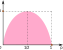
\includegraphics[width=\linewidth]{figures/shannon-distro.pdf}
\caption{Graph of Shannon distribution.\label{shannon-distro}}
 \end{wrapfigure}


Once again I emphasize that control processes should be regarded in
a dialectical unity with the random processes of disorganization. There
is a deep relationship between information theory and probability
theory. The Shannon formula \eqref{eq-3.2} illustrates this point. The
probabilistic approach provides a scientific, objective notion of
information that is free from a subjective substitution of the quantity of
information by its significance or importance.



\txthead{Information in communication channels with noise.} When information is transmitted, some loss is unavoidable. This happens because of the action of random factors, which are commonly lumped together as noise. A \redem{communication channel} for transmitting information from input set $A$ to output set $B$ is represented in \figr{comm-channel}. The information is affected by noise $P$ as it is transmitted. Suppose that $\xi$ is an input discrete random variable which may assume values $x_{1}, x_{2}, x_{3},\ldots{} , x_{N}$. with probabilities  $p_{1}, p_{2}, p_{3},\ldots{} , p_{N}$, and $\eta$ is the output variable, which may assume values $y_{1}, y_{2}, y_{3},\ldots , y_{M}$. with probabilities  $q_{1}, q_{2}, q_{3},\ldots{} , q_{M}$. Let $P_{i}(j)$ denote the probability that $\xi = y_{j}$ is the output variable if $\xi = x_{i}$ was transmitted. The probability $P_{i}(j)$ is determined by noise in the communication channel. It has been proved in information theory that the quantity of information about the random variable $\xi$ that can be obtained by observing the random variable $\eta$ is described by the formula
\begin{equation}%
I_{\eta} \, (\xi) = \sum_{i=1}^{N}\sum_{j=1}^{M} P_{i}(j) \, p_{i}  \, \log_{2} \frac{P_{i}(j)}{q_{i}}.
\label{eq-3.4}
% eq 3.4
\end{equation}
\begin{figure}[!ht]
 \centering
 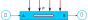
\includegraphics[width=0.8\tfwidth]{figures/comm-channel.pdf}
\caption{A communication channel for transmitting information.\label{comm-channel}}
% fig 3.7
\end{figure}
Here the information $I$ is in terms of two types of probability, the
probabilities $p_{i}$ and $q_{j}$ on the one hand and the probability $P_{i}(j)$ on the other. While the first two probabilities reflect the probabilistic nature of
the information at the input of the communication channel and that
``yes'' or ``no'' questions, the answers to which are nearly or equally
probable. Recall the question: ``Is the surname listed from 17 to 32?''
received at the output, probability $P_{i}(j)$ reflects the random nature of
the noise in the channel.

Suppose there is no noise. Then the random variable values at the
input and the output of the channel will be the same. Hence
\begin{equation}%
N = M, \,\, p_{i}= q_{i}, \,\, \text{and} \,\, P_{i}(j) = \delta_{ij},
\label{eq-3.5}
%eq 3.5
\end{equation}
where $\delta_{ij}=1$ for $i = j$ and $\delta_{ij} = 0$ for $i =1= j$.
Substituting \eqref{eq-3.5} into \eqref{eq-3.4} and noting that $\lim\limits_{z \to 0} z \, \log_{2} \, z = 0$, we get the Shannon formula. This should have been expected because when there is no noise, there is no loss of information in its transmission.


\txthead{Protection against noise in a communication channel.} There are many
sorts of communication channel. Information can be transmitted by
sound waves propagating in a medium, electric signals running along
wires, electromagnetic waves propagating in a medium or in vacuum,
etc. Each communication channel is affected by its own sorts of noise.
There are general techniques for handling noise that can be applied to
any communication channel. First of all, it is desirable to minimize the
level of noise and maximize the amount of information in the signals, so
that the signal-to-noise ratio is large. The ratio can be increased by
coding the transmitted information appropriately, e. g. transmitting it in
terms of ``symbols'' (for instance, impulses of a certain shape) which can
be distinctly identified against the background of noise. Coding a signal
increases its ``noise immunity'' or performance in terms of error
probability for the transmission.
\begin{figure}[!ht]
 \centering
 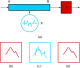
\includegraphics[width=0.8\tfwidth]{figures/noise1.pdf}
\caption{A communication channel with a filter.\label{noise1}}
% fig 3.8
 \end{figure}
 
A special measure against noise is \redem{filtering} (both \redem{smoothing} and
\redem{correlation}) the information received at the output of communication
channels. If the characteristic noise frequency in a communication
channel is substantially greater than the frequency typical for the time
change in the signal, we could use a \redem{smoothing filter} at its output to ``cut out'' the high-frequency oscillations superimposed on the signal as it was
transmitted. This is illustrated in \figr{noise1}, in which (a) is a diagram of the communication channel with a filter ($A$ is the channel input, $B$ is the
channel output, $P$ is noise, and $F$ is a smoothing filter), (b) is the signal at the input, (c) is the signal at the output before filtering, and (d) is the signal after filtering.
\begin{figure}[!ht]
 \centering
 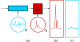
\includegraphics[width=0.8\tfwidth]{figures/noise2.pdf}
\caption{A communication channel with a filter and signal multiplier.\label{noise2}}
% fig 3.9
 \end{figure}
 
Suppose we want to find out whether the output contains a signal of
a given shape. If the signal is very different (for instance, by frequency)
from the noise background, it will be easily identified. The situation is
worse when the signal is ``masked'' by noise. Correlation filtering is
applied in these cases: a device is placed at the output which \redem{multiplies}
the output signal by the known signal. If the desired signal is present in
the output signal, the multiplication creates a very clear (large) final
(correlation) signal; otherwise no correlation signal will appear. This is
illustrated in Figure \ref{noise2}, in which (a) is a diagram of the channel ($\Lambda$ is the signal multiplier, $P$ is noise, and $S$ is the signal shape to be recognized), (b) is the multiplied signal if the recognized signal $S$ is present in the output (the correlation signal), and (c) is the multiplied signal if signal $S$ is absent in the output. Correlation filtering is used, for instance, in radar scanners to recognize the radiation signal emitted by the radar antenna.

%\clearpage

\section{Selection of Information from Noise}

\txthead{Where does information come from and some unsatisfactory answers.} Any control signal carries certain information. The signal is formed
using an algorithm which itself incorporates information, and this
algorithm was compiled in turn using information contained in other
algorithms. Thus we have a sort of relay race in which information is
transmitted from algorithm to algorithm. This idea can be illustrated by
a simple example. A teacher educates you, and in turn your teacher had
a teacher, who had a teacher, and so on.

This argument leads inevitably to the questions: Whence the ``original
information''? Whence the first algorithm? An inability (or reluctance)
to investigate scientifically the fundamental topic of where information
comes from leads to serious misconceptions.

One such misguided hypothesis is that the original information was
brought to the Earth by space travellers, who visited us in some
long-forgotten past. This hypothesis is materialistic, but it is unsatisfactory
because it begs the question of where the aliens got the
information. Modern science indicates where the information comes
from. The modern scientific answer is that there is no ``original
information'': the generation of information is a continuous and
continuing process.

\txthead{Chance at the forefront again.} The idea of information being handed
over like a relay baton in a race is simplistic. I pointed out that any
transmission of information is accompanied by loss caused by random
factors. However, random factors not only ``steal'' information, they also
generate it.

At first glance, this seems implausible. We witness the continuous
creation of information as a result of human creativity. New machines
are designed, spacecraft are launched, new books are published, and new
drugs become available: these are all a testimony to the explosive
generation of information in which everybody participates. So it would
seem strange to speak of the fundamental role of chance in generating
information.

However, consider the \redem{process of thinking}, how a problem is solved,
how an intuition appears, or how a melody or image emerges. If these
examples are too philosophical, try and think at least about \redem{associative
perception}, that is how we recognize objects and distinguish them. Just
try, and you will step into a domain of complicated links, probabilistic
relationships, chance guesses, and sudden ``revelations''. There are no
deterministic algorithms for making discoveries or solving problems.
Everything we know about the processes occurring in the brain indicates
the \redem{fundamental role} of random factors. Later I shall illustrate this by the example of \redem{perceptron}, a cybernetic device which can recognize patterns.

\txthead{Chance and selection.} How can chance generate information? How
can order appear from disorder? It turns out that the generation of
information from noise can be easily observed. You can see this for
yourself using the game of scrabble, or rather the small lettered blocks.
Put one block with each letter of the alphabet into a bag, mix them, and
take one out at random. Write down each randomly taken letter and
return the block to the bag. Each time shake the bag. This simple
generator of random letters can be used to generate a long chaotic
string. If you look closely, you will find some three-letter words, perhaps
even words with more letters. Information is being generated from noise.

My son, for example, helped me do an experiment and in a string of
300 random letters found nine three-letter words and two four-letter.
This argument leads inevitably to the questions: Whence the ``original
information''? Whence the first algorithm? An inability (or reluctance)
words. The more letters there are in a word, the smaller the probability
of generating the word from ``letter noise''. The generation of a sentence,
let alone a line from a well-known work, is less probable. Nonetheless,
the probability of doing is nonzero, and so there is the possibility of any
information being generated randomly from noise.

Thus, we can say (although this sounds strange) that \redem{chance generates
information by chance}. The greater the information, the smaller the
probability of its random generation. That random information can be
generated does not solve the basic problem. This randomly generated
information must be detected from the enormous flow of meaningless
``signals''. In other words, the \redem{information must be selected from the noise}. In the example of taking lettered blocks out, the information is selected
from the noise by the person who wrote out the letters and looked
through the string.

\txthead{Selection amplifier} Is it possible to use chance conscientiously to
generate information? It is, so long as we \redem{amplify the selection}.

You can do a simple experiment to demonstrate the amplification of
selection using the random letter generator described above. In order to
amplify the selection, we take into account the frequency with which
letters appear in each word. Letter frequencies in English are often given
when you buy a commercial game of scrabble. To allow for the frequencies,
first eliminate the rare letters, e. g. $Z, Q, J, V, X$ and add extra
blocks with frequent letters, e. g. four blocks with $E$ and $T$, three with $A,
I, O, L, N, G, R, S$, two with $D, U,$ and one of all the rest. I cannot
vouch that this selection is optimal, in a similar experiment I found 21
three-letter words, 4 four-letter words and 1 five-letter word in
a succession of 300 random letters.

In order to amplify the selection still greater, we should use \redem{words}
rather than \redem{letters}. It is curious that a similar device was suggested in
the early $18^{\text{th}}$ century by the English satirist Jonathan Swift in
Gulliver's travels. When Gulliver visited the Academy in Lagado (the
capital of an imaginary kingdom), he met a professor who had an
interesting apparatus. Swift wrote:
\begin{quote}
``He then led me to the frame, about the sides whereof all his pupils
stood in ranks. It was twenty feet square, placed in the middle of the
room. The super faces were composed of several bits of wood, about the
bigness of a die, but some larger than others. They were all linked together
by slender wires. These bits of wood were covered on every square
with papers pasted on them, and on these papers were written all the
words of their language in their several moods, tenses, and declensions,
but without any order. The professor then desired me to observe, for he
was going to set his engine at work. The pupils at his command took,
each of them, hold of an iron handle, there were forty fixed around the
edges of the frame, and given then a sudden turn, the whole disposition
of the word was entirely changed. He then commanded six and thirty of
the lads to read the several lines softly as they appeared on the frame;
and where they found three or four words together they might make part of a sentence, they dictated to the four remaining boys who were scribes. This work was repeated three or four times, and at every turn the engine was so contrived, that the words shifted into new places, as the square bits of wood moved upside down.''
\end{quote}
True, Swift wrote satirically, laughing about such inventions.
However, why should we not believe that a talented popular-science
writer disguised himself behind mask of a satirist so as not to be
laughed at and misunderstood by his contemporaries?

What seemed absurd and laughable in the $18^{\text{th}}$ century has now
become the subject of scientific investigation in the mid-$20^{\text{th}}$ century. The English scientist W. Ross Ashby suggested a cybernetics device in
the early 1950s which could be a \redem{selection amplifier}. Ashby called it an
\redem{intelligence amplifier}. A diagram of this amplifier is given in \figr{selection-amp}.

\begin{wrapfigure}{O}{\mfwidth}
 \centering
 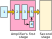
\includegraphics[width=\linewidth]{figures/selection-amp.pdf}
 \caption{A selection amplifier.\label{selection-amp}}
% fig 3.10
 \end{wrapfigure}
Noise generator 1 supplies ``raw material'' to the first stage of the
amplifier. The noise converter 2 produces various random variants of
the subjects to be selected. The selection is performed in unit 3 in
compliance with criteria of selection put into this device. In a concrete
case, if the result of a selection meets a criterion, control unit 4 opens
valve 5 and lets the selected information into the converter of the next
stage of the amplifier. One can easily imagine that the first stage of the
amplifier, supplied with random letters, selects separate randomly
emerging words or separate typical syllables; the second stage of the
amplifier selects word combinations; the third stage selects sentences,
the fourth stage selects ideas, etc.

\txthead{Random search-related self-organization. The homeostat.} Suppose
a system is in a state which a allows it to carry out certain functions. Let
us call this state \redem{normal}. It corresponds to external. conditions in which
the system operates. Suppose these conditions change all of a sudden,
and the result is that the system departs from the normal state. The new
conditions correspond to a new normal state. It is desirable to transfer
and where they found three or four words together they might make
part of a sentence, they dictated to the four remaining boys who were
scribes. This work was repeated three or four times, and at every turn
the system to this new state. How is it to be done? Information is
needed firstly on the new state, and, secondly, on how the transition of
the system to the new state can be carried out. Since the change in the
environment is random in nature, we know neither the new normal state
nor how to organize a transition to it. A \redem{random search} may help in
such situations. This means that we should randomly change the
system's parameters until it randomly matches the new normal state,
which can be immediately recognized by monitoring the system's
behaviour.

\begin{wrapfigure}[15]{O}{\mfwidth}
 \centering
 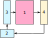
\includegraphics[width=0.9\linewidth]{figures/homeostat.pdf}
\caption{A homeostat is a device which possessed the property of
self-organization on the basis of random search.\label{homeostat}}
% fig 3.11
 \end{wrapfigure}

It can be said that the process of random search generates the
information needed to transfer the system to the new normal state. This
is nothing else but the \redem{selection of information from noise} about which we have been talking. The selection criterion here is the change in the
system's behaviour: once in the new normal state, the system ``calms
down'' and starts functioning normally.

In 1948 Ashby designed a device which possessed the property of
self-organization on the basis of random search. He called the device
a \redem{homeostat}. A diagram of a homeostat is shown in \figr{homeostat}.

A homeostat is often compared to a sleeping cat. If the cat is bothered,
it wakes up, chooses a new more comfortable position, and goes to sleep
again. A homeostat behaves in a similar manner: when it is ``woken up'',
it carries out random search for new values for its parameters, and when
it finds them, it ``goes to sleep'' again.

\begin{wrapfigure}[20]{O}{\mfwidth}
 \centering
 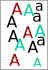
\includegraphics[width=0.9\linewidth]{figures/fonts.pdf}
\caption{A selection of different ways of writing letter A.}
\label{fonts}
% fig 3.12
 \end{wrapfigure}

System 1 in \figr{homeostat} may be either in a stable or unstable state.
Without going into detail, let me note that system 1 consists of four
electromagnets whose cores can move and control the rheostats which
control the voltages across the electromagnets. Therefore, the rotation
angle of each electromagnet is dependent on all the other ones. These
angles are the parameters of this dynamic system. The magnet cores do
not rotate when the system is in a stable state. However, if an external
disturbance takes the system out of its stable state, control unit
2 switches on generator 3 of random changes of parameters, and the
random search starts. Once system 1 finds a stable state (by chance),
the system to this new state. How is it to be done? Information is
needed firstly on the new state, and, secondly, on how the transition of
the system to the new state can he carried out. Since the chance in the
unit 4 having verified the stability sends a signal to control unit 2, which
switches off the random parameter generator 3.

\section{On the Way to a Stochastic Model of the Brain}

\txthead{The pattern recognition problem.} We do not commonly think about the
brain's ability to \redem{recognize} patterns, although it is amazing. Several
characters differing in size, shape, and line breadth are shown in
\figr{fonts}. Despite this, we immediately recognize the same character, the letter $A$, in every image. It is still more amazing when there is a crowd
of variously dressed people with poorly distinguishable faces (because of
the distance) and yet we usually manage to distinguish between men and
women without error.

The ability to recognize patterns is called \redem{associative perception}, i.e.
when certain general, characteristic features are perceived while other
more individual aspects recede into the background. Is associative
perception possible for a machine? Is it possible to simulate the
processes occurring in the brain and relate them to pattern recognition?
These questions were answered in the affirmative in 1960 when the
American scientist F. Rozenblutt designed a device he called
a \redem{perceptron}.

\txthead{What is a perceptron?} A perceptron can be regarded as an
oversimplified model of the eye-brain system. The role of the eye, or,
more accurately, the retina of the eye, is played by a grid consisting of
a large number of \redem{photoelectric cells}, or \redem{receptors}. Each receptor converts the light incident on it into electric signals which are collected by the analysis unit within the perceptron. Before going into detail on
the perceptron, let me make two fundamental points. Firstly, the
relations between the receptors and the perceptron's internal units which
process the information recorded by receptors should not be rigidly
defined. If they were so defined, the signals from the images shown in
\figr{perceptron1} (a) and (b) would be ``perceived'' by the perceptron as
different patterns (only five excited receptors shown in red coincide in
these images), while the images in \figr{perceptron1} (a) and (c) would be
``perceived'', by contrast, to be the same pattern because there are 28
excited receptors in common. In reality, a perceptron should ``perceive''
the images in \figr{perceptron1} (a) and (b) as the same pattern while those in \figr{perceptron1} (a) and (c) as different patterns. Thus, we must accept that the internal relations in a perceptron should be \redem{random}. They have to be \redem{probabilistic} relations.

\begin{figure}[!ht]
 \centering
 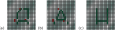
\includegraphics[width=\tfwidth]{figures/perceptron1.pdf}
\caption{Signals and their interpretations by a perceptron.\label{perceptron1}}
% fig 3.13
 \end{figure}
Secondly, the random nature of these relations suggests the \redem{adjustment}
of the perceptron to the patterns being recognized. A perceptron should
he presented with different images of the recognized patterns in turn
(and several times), and we should \redem{teach} it, the perceptron's parameters
being adjusted as needed in the process. A perceptron should take into
account its progress at each stage (at each presentation of the image), so
a perceptron should have a memory.

Considering both these points, we can define perceptrons to be
devices which have a memory and a random structure of the links
between its units. A perceptron can be thought of as a simplified model
of the brain, and this model is promising because it is \redem{probabilistic}, or,
in other words, \redem{stochastic}. Some scientists believe that stochastic models will be best able to simulate the processes occurring in the brain.
Various sorts of perceptron have been designed. Below we shall
consider a simple perceptron which can distinguish two patterns.

\txthead{The arrangement of the simplest perceptron.} A diagram of this
perceptron is given in \figr{perceptron2}. Here the $S_{i}$, are photoelectric cells (receptors), the $I_{k}$ are phase inverters, which change the sign of the electric voltage, the $A_{j}$ are associative units ($A$-units), the A. $\lambda_{j}$ are amplifiers with varying gain factors, $\Sigma$ is a summator, and $R$ is the receiver, Suppose that the total number of receptors $S_{i}$, is $N$, $(i = 1, \, 2, \, 3, \ldots{} , N)$. In the first models, $N$ was $20 \times 20 = 400$ receptors. The number of inverters is not fixed in that it can be different in different copies of the same device. The total number of associative units $A_{j}$ and amplifiers $\lambda_{j}$ equals $M \,\, (j = 1, \, 2, \ldots{} ,\, M)$. The receptors are wired to the $A$-units either directly or via the inverters. It is essential that the choice of which receptor is connected to which $A$-unit and the selection of the potential sign are random. Thus when a circuit is being assembled, the wires connecting the receptors to the $A$-units are soldered together \redem{randomly}, for instance, in accordance with instructions from a random
number generator.

\begin{figure}[ht]
 \centering
 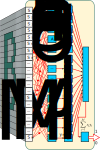
\includegraphics[width=.68\tfwidth]{figures/perceptron2.pdf}
\caption{Schematic diagram of the simplest perceptron.\label{perceptron2}}
% fig 3.13
 \end{figure}
 
Suppose that an image is projected onto the perceptron's sensor grid.
Since the intensity of the light at each point is different, some of the
receptors will be excited, generating a logic signal of 1, while others will
not, generating an electric signal of 0 at the output of the receptor. If the
signal passes through an inverter, a 1 is transformed into a $-1$. The
system of random links transmits the signals from the receptors to the
$A$-units. Each $A$-unit algebraically adds up the signals at its input. If the
sum is above a threshold, the output of the $A$-unit goes to logic + 1,
otherwise it goes to logic 0. Let us designate the signals leaving the
$A$-units $y_{j}$. Each $y_{j}$ is either + 1 or 0. The signal at the output of unit $A_{j}$ goes to the input of amplifier $\lambda_{j}$ and the amplifier transforms signal $v_{j}$ to a signal $\varkappa_{j} y_{j}$: The gain factor $\varkappa_{j}$ may vary both in absolute value and in sign. The signals from all the amplifiers are summed up in the summator $\Sigma$, and hence we get 
\begin{equation*}%
\sum_{j= 1}^{M} \varkappa_{j} y_{j}.
\end{equation*}
Then it is sent to the input of the $R$-unit, which checks its sign. If
$\sum_{j} \varkappa_{j} y_{j} \geqslant 0$, the $R$-unit output is + 1, otherwise the $R$-unit output is 0.

This perceptron is designed to recognize only two patterns.
Irrespective of the concrete images of the patterns, the perceptron will
respond to one pattern with an output signal of + 1 and with a signal
of 0 to the other. The perceptron must \redem{learn} this ability.

\txthead{Teaching a perceptron.} Let us call the two patterns $B$ and $C$. Suppose pattern $B$ corresponds to an output signal of + 1 and pattern $C$ to an output signal of 0. Suppose $\varkappa_{1}, \varkappa_{2}, \varkappa_{3},\ldots{} ,  \varkappa_{j},\ldots{}, \varkappa_{M}$ are the perceptron's gain factors before it is taught. Let us designate this ordered set $\{ \varkappa \}$. To teach the perceptron, we present it with an image of pattern $B$. This will excite a certain set of $A$-units, i. e. we get a succession of signals $y_{1}, y_{2}, y_{3},\ldots{} ,y_{j},\ldots{} , y_{M}$, or, in short, $\{ y \}$. Now suppose the sum $\sum_{j} \varkappa_{j} y_{j} $ is
non-negative, so the perceptron's output signal is + 1. If so, then
everything is true, and we can present the perceptron with a second
image of pattern $B$. The second image will excite a new set of $A$-units,
i.e. a new succession of signals $\{ y' \}$. The set of gain factors $\{ \varkappa \}$ remains yet the same, but the sum $\sum_{j} \varkappa_{j}' y_{j}' $ may be negative, and then the signal at the perceptron's output will be 0. This is not good, and therefore the perceptron is ``discouraged'': the gain factors of the excited $A$-units are incremented by, say, unity, so that a new set of gain factors $\{ \varkappa '\}$ ensures that the sum $\sum_{j} \varkappa_{j}' y_{j}' $ is non-negative. Now the perceptron responds correctly to the second image of pattern $B$. But what about the first image? The set of gain factors has been changed, so that the sign of the sum $\sum_{j} \varkappa_{j}' y_{j} $ may be changed. We present the perceptron with the first image of pattern $B$ again and identify the sign of the sum $\sum_{j} \varkappa_{j}' y_{j} $  by the output signal.

If the sum is non-negative, we are satisfied because the set of gain
factors $\{ \varkappa' \}$ has caused the perceptron to respond correctly to both the first and the second images of pattern $B$. Now we can present the
perceptron with a third image of pattern $B$. If the sum is negative, the
gain factors of the excited $A$-units should be incremented by unity again
(set $\{ \varkappa' \}$ is replaced by set $\{ \varkappa'' \}$), and so on.

Gradually, by varying the set of gain factors step by step, we will find
a set of factors such that the perceptron will produce a signal of + 1 for
any presented image of pattern $B$. However, our job is not yet over. It is
quite possible that after many increments of the various gain factors, the
perceptron will produce a + 1 signal for both pattern $B$ and pattern
$C$ images. However, the perceptron should produce a + 1 signal for all
pattern $B$ images and a 0 signal for all pattern $C$ images. This means
that while the perceptron is being taught, we should alternate between
both patterns and when presenting an image of pattern $C$, we should (if
need be) decrement rather than increment the gain factors of the excited
$A$-units to get $\sum x y$ below zero.

Ultimately, we will find a set of gain factors  $\{ \varkappa^{0} \}$ such that the perceptron will always recognize patterns $B$ and $C$. Suppose  $\{ y(n) \}$ is the set of excited $A$-units corresponding to an $n$th image of pattern
$B$ and  $\{ Y(m) \}$ is a set corresponding to an $m$th image of pattern $C$. The $M$ gain factors $\{ \varkappa^{0} \}$ should be such that 
\begin{equation*}
%\begin{split}
\sum_{j= 1}^{M} \varkappa^{0}_{j} y_{j} (n)  \geqslant 0 \,\, \text{for all} \,\, n \,\, \text{and} \,\,
\sum_{j= 1}^{M} \varkappa^{0}_{j} y_{j} (m)  \geqslant 0 \,\, \text{for all} \,\, m
%\end{split}
\end{equation*}

The teaching (and the learning) is over when such gain factors have been found.

\txthead{Conclusion.} In concluding this chapter, I went to emphasize the main
point, i.e. the deep, intrinsic relationship between \redem{information theory} and \redem{probability theory}. The very notion of information is underlain by
probability. And this is natural because control processes and random
processes are always \redem{dialectically united}. Randomness both ``steals''
information and generates it, because the most complicated information
devices are fundamentally based on random internal structures.

We see that the phrase ``the world is built on probability'', which is
the title of this book, has a deeper meaning. Mankind lives and acts in
a world filled with information. This information arises by nature
through probability and, moreover, is created in probabilistic processes.
Thus, a \redem{world filled with information} is naturally a \redem{world built on
probability}.
%%% Local Variables:
%%% mode: latex
%%% TeX-engine: xetex
%%% TeX-master: "twibop2"
%%% End:
